\chapter{Auswertung}\label{cha:auswertung}
Dieses Kapitel befasst sich mit der Genauigkeit der Bestimmung der Elementarladung. Zunächst wird ein Überblick auf die im Experiment erhaltenen Daten gegeben. In \autoref{tab:ergebnisse} sind die relevanten Messgrössen aufgeführt, nämlich die Steig- und Fallgeschwindigkeiten, der Radius, die Masse sowie die Ladung der Tröpfchen. Eine vollständige Übersicht der \textbf{Messwerte ist im Anhang zu finden}, wobei auch Messungen, die nicht ausreichend präzise waren, berücksichtigt werden. Diese wurden jedoch nicht in den Berechnungen einbezogen.

In der Fehlerrechnung (\autoref{sub:fehler}) wurde die Maturaarbeit von Herr Brenner \parencite{maturaarbeitBrenner} zur Hilfestellung der Funktionsweise einer Fehlerrechnung dazugezogen.

\section{Ausgehobene Daten}\label{sec:aushebungDaten}
Die Daten können nun in einem Punktdiagramm eingefügt werden, wobei die Y-Achse die Ladung der Tröpfchen und die X-Achse die jeweilige Nummer der Messung darstellt. Das Diagramm wurde mit Microsoft Excel erstellt und wird im Folgendem dargestellt.

\begin{figure}[h]
	\centering
	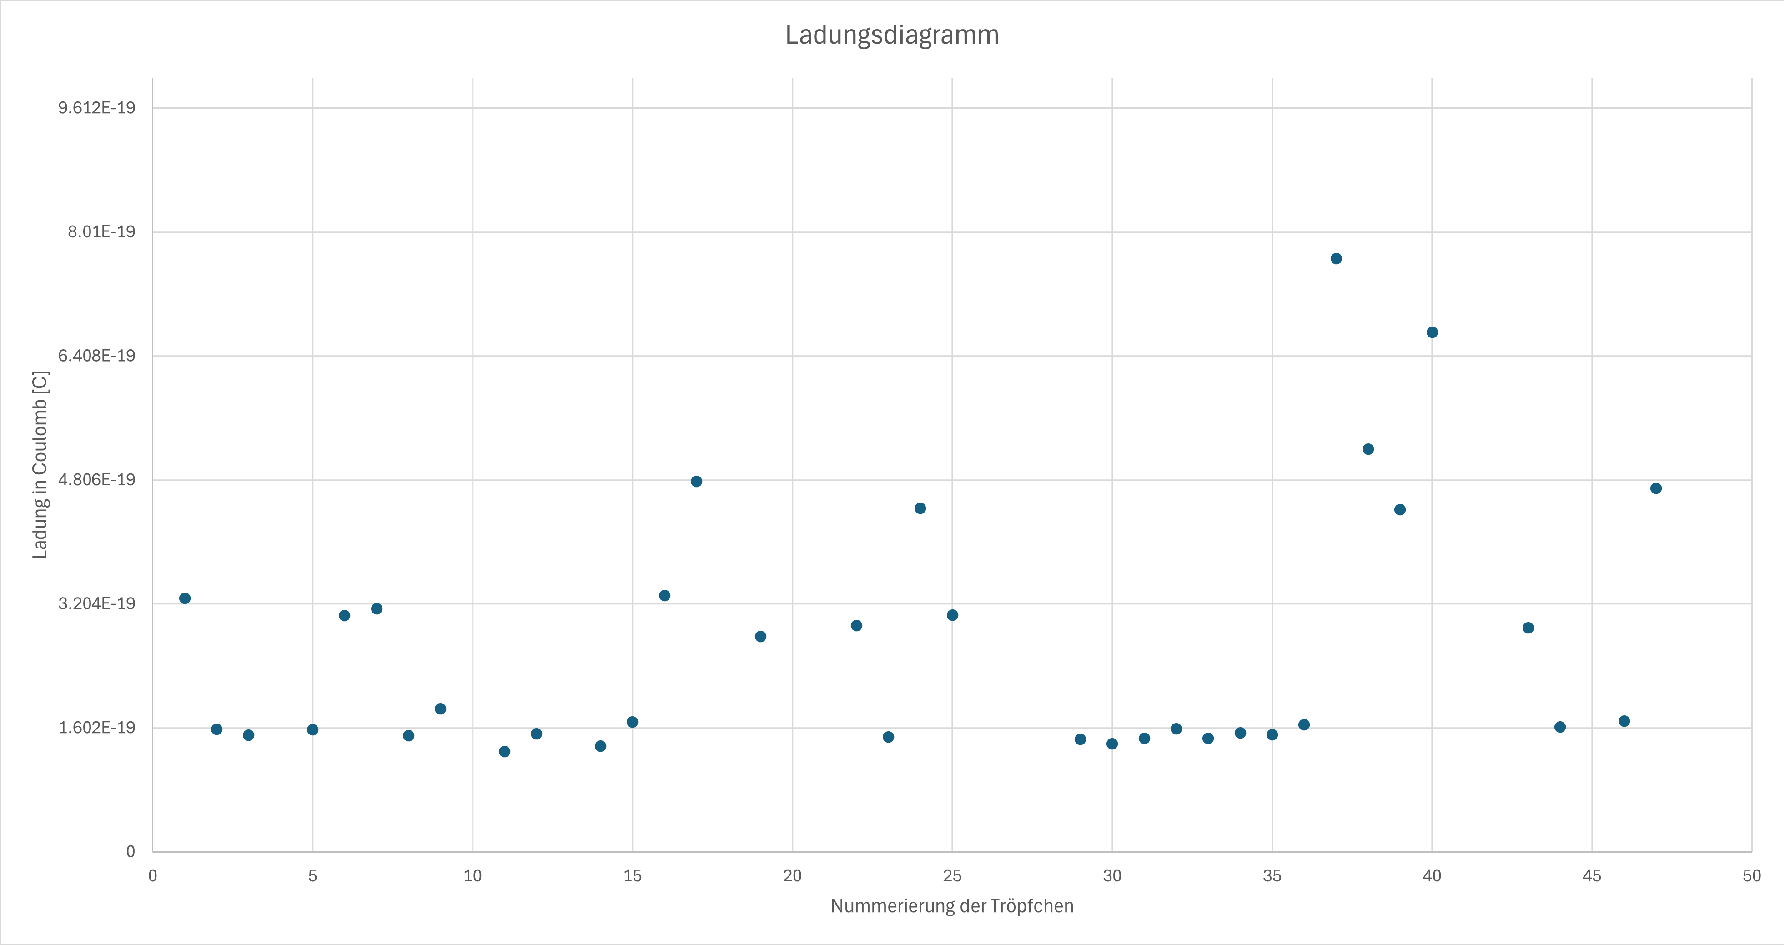
\includegraphics[width=\textwidth]{bilder/pdf/LadungsdiagrammOhne.pdf}
	\caption{Ladungsdiagramm ohne Fehlerrechnung}
	\label{fig:ladungsdiagrammOFehlerrechnung}
\end{figure}

\noindent Die Abstände auf der Y-Achse sind nicht zufällig gewählt, sondern entsprechen exakt einer Elementarladung. Anhand dieses Diagramms kann die Anzahl der Elementarladungen jedes einzelnen Tröpfchens abgelesen werden. Es war überraschend, wie präzise das Experiment verlief. Die Ladungen der Tröpfchen ordnen sich klar in Stufen, was während des Experimentierens nicht zu erwarten war. Weitere Details zur Genauigkeit der Messungen werden in \autoref{sec:genauigkeitAuswertung} behandelt, indem eine Fehlerrechnung zur Bewertung der Resultate gemacht wird. 

\section{Das Ergebnis}\label{sec:ergebnis}
In \autoref{tab:ergebnisse} kann nun eine weitere Spalte eingefügt werden, die die Anzahl der Elementarladungen $n$ angibt. Nachdem diese hinzugefügt wurde, sieht die Tabelle für die ersten 10 Zeilen wie folgt aus:

\begin{table}[H]
	\centering
	\begin{tabular}{llllll|l}
		\toprule
		Nr. & $v_{rise}$ [$m/s$] & $v_{fall}$ [$m/s$] & Radius [$m$] & Masse [$kg$]  & Ladung [$C$]& Anzahl (n) \\
		\midrule
		1 &$\mathrm{2.01 \cdot 10^{-04}}$ & $\mathrm{2.12 \cdot 10^{-05}}$ & $\mathrm{4.04 \cdot 10^{-07}}$ & $\mathrm{2.45 \cdot 10^{-16}}$ & $\mathrm{3.27 \cdot 10^{-19}}$ & 2\\
		2 &$\mathrm{8.46 \cdot 10^{-05}}$ & $\mathrm{2.16 \cdot 10^{-05}}$ & $\mathrm{4.08 \cdot 10^{-07}}$ & $\mathrm{2.53 \cdot 10^{-16}}$ & $\mathrm{1.59 \cdot 10^{-19}}$ & 1\\
		3 &$\mathrm{8.68 \cdot 10^{-05}}$ & $\mathrm{1.98 \cdot 10^{-05}}$ & $\mathrm{3.90 \cdot 10^{-07}}$ & $\mathrm{2.20 \cdot 10^{-16}}$ & $\mathrm{1.51 \cdot 10^{-19}}$ & 1\\
		4 &$\mathrm{8.91 \cdot 10^{-05}}$ & $\mathrm{2.04 \cdot 10^{-05}}$ & $\mathrm{3.96 \cdot 10^{-07}}$ & $\mathrm{2.31 \cdot 10^{-16}}$ & $\mathrm{1.58 \cdot 10^{-19}}$ & 1\\
		5 &$\mathrm{1.97 \cdot 10^{-04}}$ & $\mathrm{1.98 \cdot 10^{-05}}$ & $\mathrm{3.89 \cdot 10^{-07}}$ & $\mathrm{2.18 \cdot 10^{-16}}$ & $\mathrm{3.05 \cdot 10^{-19}}$ & 2\\
		6 &$\mathrm{1.98 \cdot 10^{-04}}$ & $\mathrm{2.04 \cdot 10^{-05}}$ & $\mathrm{3.96 \cdot 10^{-07}}$ & $\mathrm{2.31 \cdot 10^{-16}}$ & $\mathrm{3.14 \cdot 10^{-19}}$ & 2\\
		7 &$\mathrm{9.33 \cdot 10^{-05}}$ & $\mathrm{1.84 \cdot 10^{-05}}$ & $\mathrm{3.74 \cdot 10^{-07}}$ & $\mathrm{1.95 \cdot 10^{-16}}$ & $\mathrm{1.50 \cdot 10^{-19}}$ & 1\\
		8 &$\mathrm{1.26 \cdot 10^{-04}}$ & $\mathrm{1.71 \cdot 10^{-05}}$ & $\mathrm{3.61 \cdot 10^{-07}}$ & $\mathrm{1.74 \cdot 10^{-16}}$ & $\mathrm{1.85 \cdot 10^{-19}}$ & 1\\
		9 &$\mathrm{1.12 \cdot 10^{-04}}$ & $\mathrm{1.23 \cdot 10^{-05}}$ & $\mathrm{3.01 \cdot 10^{-07}}$ & $\mathrm{1.01 \cdot 10^{-16}}$ & $\mathrm{1.29 \cdot 10^{-19}}$ & 1\\
		10 &$\mathrm{1.30 \cdot 10^{-04}}$ & $\mathrm{1.29 \cdot 10^{-05}}$ & $\mathrm{3.08 \cdot 10^{-07}}$ & $\mathrm{1.09 \cdot 10^{-16}}$ & $\mathrm{1.53 \cdot 10^{-19}}$ & 1\\
		\bottomrule
		&&&&& $2.031 \cdot 10^{-18}$ & 13 \\
	\end{tabular}
	\caption{Ergebnisse mit Anzahl Ladungen}
	\label{tab:anzahlLadung}
\end{table}
\par
\noindent Die Anzahl der Elementarladungen wird addiert, was zu einer Summe von 13 Elementarladungen führt. Anschliessend werden die Ladungen summiert, was den Wert $2.031 \cdot 10^{-18}$ Coulomb ergibt. Das arithmetische Mittel dieser beiden Messwerten lautet dann: $\frac{2.031 \cdot 10^{-18}}{13} \ = \ 1.56 \cdot 10^{-19} Coulomb$. 

Wenn dieser Vorgang für alle Werte in der Tabelle wiederholt wird, ergibt sich eine Anzahl von 60 Elementarladungen und eine Gesamtsumme von $9.313 \cdot 10^{-18}$ Coulomb. Das Mittel dieser Werte führt zu einem Ergebnis für die Elementarladung von:

\begin{equation}\label{eq:ergebnis}
	\frac{9.313 \cdot 10^{-18}\ C}{60} \ = \ 1.552 \cdot 10^{-19}\ C
\end{equation}

\section{Die Genauigkeit}\label{sec:genauigkeitAuswertung}
Die Genauigkeit eines solchen Experimentes kann nur durch eine gründliche Fehlerrechnung bewertet werden. Im Folgenden wird die Fehlerrechnung erläutert, um den Einfluss der Fehlerquellen auf das Ergebnis hervorzuheben. Für jede relevante Grösse wird sowohl der absolute als auch der relative Fehler berechnet. Diese Fehler werden anschliessend miteinander kombiniert, um die Gesamtunsicherheit der Messergebnisse zu ermitteln.

In jedem Experiment treten Fehler auf, die entweder durch die Messinstrumente oder durch den Experimentieraufbau verursacht werden. Ein Beispiel für solche systematischen Fehler ist die mögliche Fehlkalibrierung des Multimeters oder eine ungenaue Erstellung des Fadenkreuz, bei dem die Gitternetzlinien nicht exakt 0,5 mm voneinander entfernt sind. Systematische Fehler können durch präzise Kalibrierung der Geräte und sorgfältige Vorbereitung des Experiments minimiert werden.

Zusätzlich gibt es auch die zufälligen Fehler, die durch unkontrollierbare Schwankungen während des Experiments auftreten. Beispiele hierfür sind die Reaktionszeit beim Starten der Stoppuhr, der Blickwinkel beim Beobachten der Tröpfchen oder auch Faktoren wie Temperatur- und Luftdruckschwankungen während des Experiments. Diese Fehler sind schwieriger zu eliminieren, können jedoch durch wiederholte Messungen und der Berechnung von Mittelwerten verringert werden, wodurch die zufälligen Fehler minimiert werden.

\subsection{Fehlerrechnung}\label{sub:fehler}
Zuerst müssen für alle Messgrössen die absoluten Fehler festgelegt werden. Diese können entweder geschätzt werden oder hängen von der Genauigkeit des jeweiligen Messgeräts ab.

\begin{table}[h]
	\begin{center}
		\begin{tabular}{l|lll}
			                             & Messwert     & absoluter Fehler     & relativer Fehler [\%] \\ \toprule
			Elektrisches Feld $[V/m]$    & zsmg. Grösse &                      & 0.68\%                \\
			Steigzeit $[s]$              & 3.7          & 0.1                  & 2.70\%                \\
			Sinkzeit $[s]$               & 32.6         & 0.1                  & 0.31\%                \\
			Distanz $[m]$                & 0.0005       & 0.00001              & 2.00\%                \\
			Steiggeschwindigkeit $[m/s]$ & zsmg. Grösse &                      & 4.70\%                \\
			Sinkgeschwindigkeit $[m/s]$  & zsmg. Grösse &                      & 2.31\%                \\
			Luftdruck $[Pa]$             & 94000        & 1000                 & 1.06\%                \\
			Zähigkeit $[Ns/m^2]$         & 0.00001818   & 0.00000001           & 0.05\%                \\
			Dichte $[kg/m^3]$            & 886          & 1                    & 0.11\%                \\
			Fallbeschleunigung $[m/s^2]$ & 9.81         & 0.05 & 0.51\%                \\
			Konstante b                  & 0.0082       & 0.00001              & 0.12\%
		\end{tabular}
	\end{center}
	\caption{Fehlertabelle Messgrössen}
	\label{tab:messabsFehler}
\end{table}

\noindent Zuerst wird der Fehler für den Radius berechnet:
\begin{equation*}\label{eq:fehlerRadius}
	\begin{split}
		Fehler_{Radius} & \ = \ \sqrt{\left( \frac{b}{2p}\right)^2 + \frac{9\eta v_f}{2\rho g}} - \frac{b}{2p} \ = \ \sqrt{\frac{9\eta v_f}{2\rho g}} - \frac{b}{2p} \\
		                & \ = \ \sqrt{\frac{0.05\% \cdot 2.31\%}{0.11\% \cdot 0.51\%}} - \frac{0.12\%}{1.06\%} \ = \ 1.49\% - 1.18\%                                              \\
		                & \ = \ 2.67\%
	\end{split}
\end{equation*}

\noindent Anschliessend kommt der Fehler für die Masse:
\begin{equation*}\label{eq:fehlerMasse}
	Fehler_{Masse} \ = \ \frac{4}{3} \pi \cdot a^3 \cdot \rho \ = \ (2.67\%)^3 \cdot 0.11\% \ = \ 8.12\%
\end{equation*}

\noindent Zuletzt erfolgt die Fehlerrechnung für die Ladung:
\begin{equation*}
	\begin{split}
		Fehler_{Ladung} & \ = \ \frac{mg(v_f + v_r)}{Ev_f} \ = \ \frac{8.12\% \cdot (4.70\% + 2.31\%)}{0.68\% \cdot 2.31\%} \\
		& \ = \ \frac{11.63\%}{2.99\%} \ = \ 14.62\%	
	\end{split}
\end{equation*}

\noindent Dieser Fehler für den Radius kann nun im Ladungsdiagramm berücksichtigt werden. Das Diagramm sieht dann wie folgt aus.

\begin{figure}[h]
	\centering
	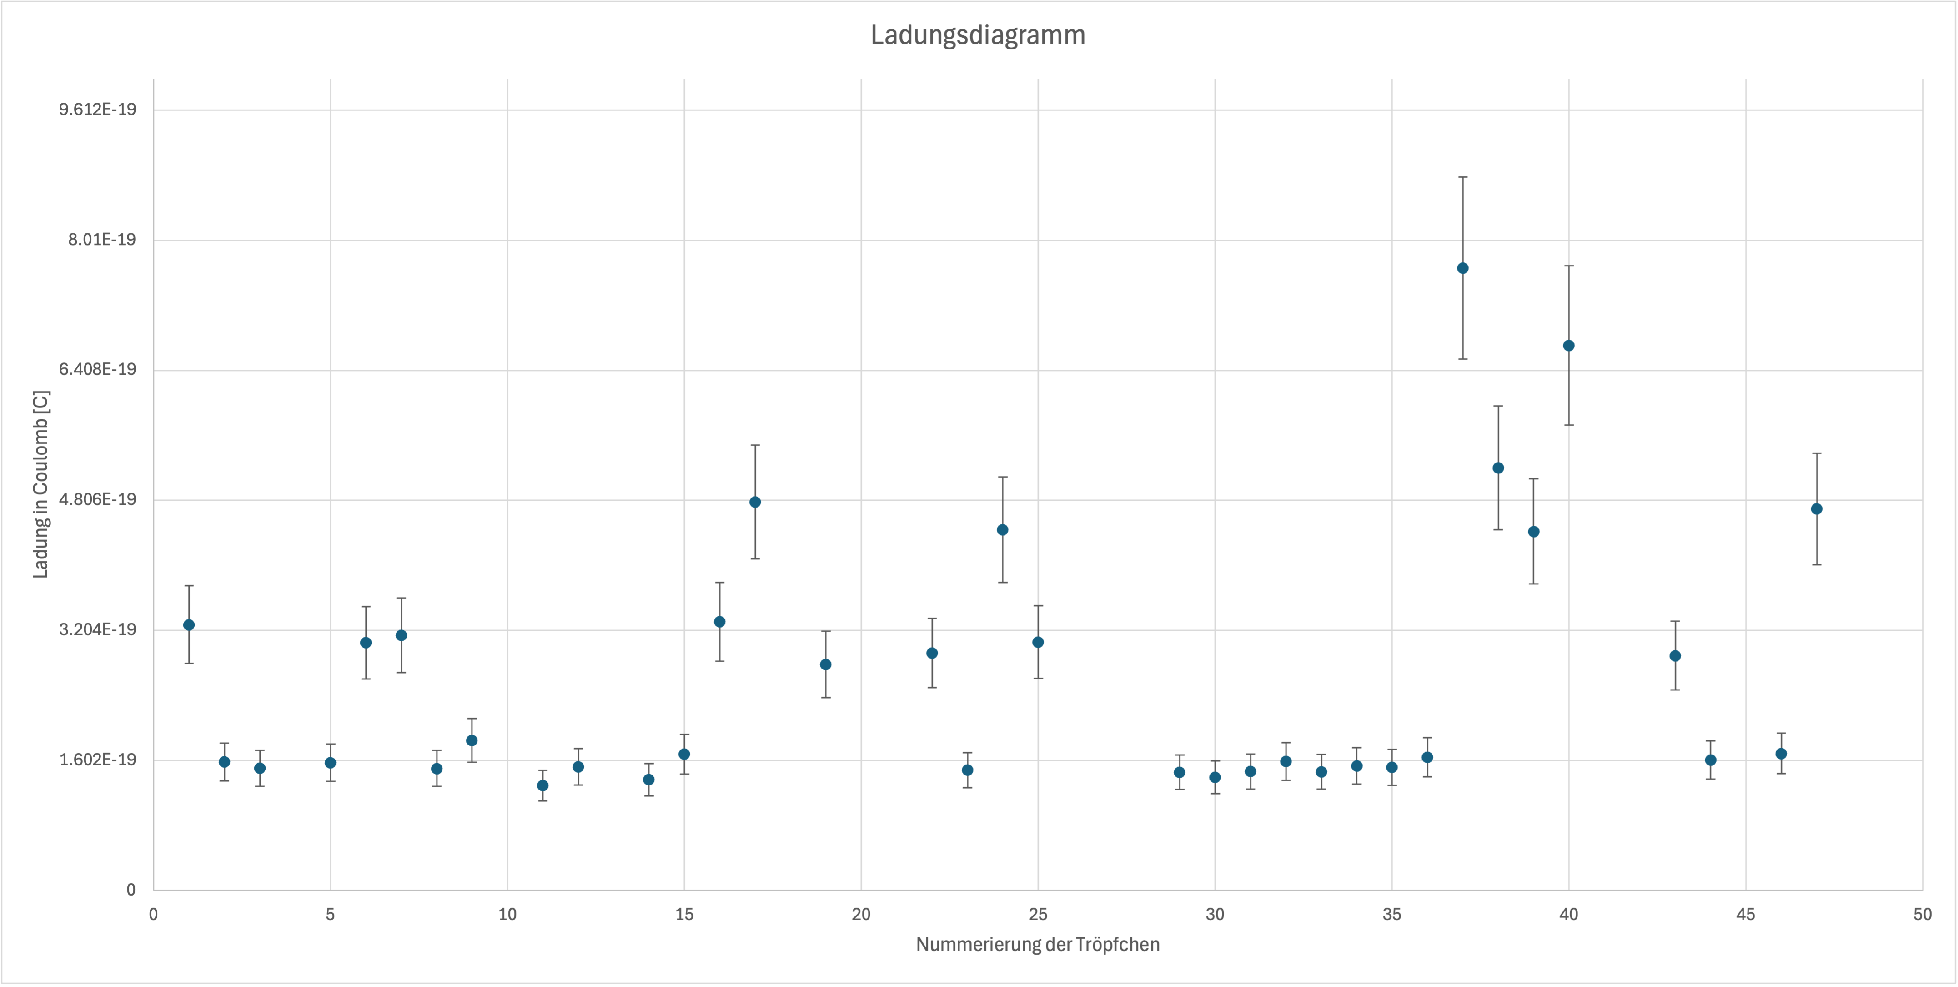
\includegraphics[width=\textwidth]{bilder/pdf/LadungsdiagrammMitNeu.pdf}
	\caption{Ladungsdiagramm mit Fehlerrechnung}
	\label{fig:ladungsdiagrammMFehlerrechnung}
\end{figure}

\subsection{Schlussfolgerung des Ergebnis}\label{sub:schlussfolgerung}
Während des gesamten Experiments traten keine unplausiblen Werte auf, die eine deutlich zu hohe oder niedrige Ladung anzeigten. 

Mit diesem Schritt wird das Ergebnis des Millikan-Versuchs vollständig abgeschlossen. Das Diagramm, das zusammen mit den Fehlerberechnungen erstellt wurde, zeigt deutlich, dass alle Tröpfchen einer bestimmten Ladungsstufe zugeordnet werden können. Dies war während des Experiments zunächst nicht abzusehen. Erstaunlich ist, dass trotz der Vielzahl an Messgrössen, die jeweils mit unterschiedlichen Fehlerquellen behaftet sind, der berechnete Wert mit 19 Dezimalstellen konstant bleibt und im Bereich der theoretisch erwarteten Elementarladung liegt. Dies verdeutlicht die hohe Präzision des Experiments und die Stabilität des Ergebnisses, selbst bei der Auswertung der zahlreichen Messungen. \\

\noindent Der Fehler für das Messergebnis lautet wie folgt.

$$
\frac{\Delta Fehler}{Messwert} \ = \ rel. Fehler \ = \ \frac{\pm \ 5.002 \cdot 10^{-21}\ C}{1.552 \cdot 10^{-19}\ C} \ = \ 3.22 \%
$$

\noindent Wie in dieser Rechnung gezeigt, liegt der relative Fehler des Messergebnis im Rahmen des Fehlers vom Experiment. 





\begin{table}
\caption{Ergebnisse der Berechnung}
\label{tab:ergebnisse}
\begin{tabular}{lllll}
\toprule
v_rise & v_fall & Radius & Masse & Ladung \\
\midrule
2.01 \times 10^{-04} & 2.12 \times 10^{-05} & 4.04 \times 10^{-07} & 2.45 \times 10^{-16} & 3.27 \times 10^{-19} \\
8.46 \times 10^{-05} & 2.16 \times 10^{-05} & 4.08 \times 10^{-07} & 2.53 \times 10^{-16} & 1.59 \times 10^{-19} \\
8.68 \times 10^{-05} & 1.98 \times 10^{-05} & 3.90 \times 10^{-07} & 2.20 \times 10^{-16} & 1.51 \times 10^{-19} \\
8.91 \times 10^{-05} & 2.04 \times 10^{-05} & 3.96 \times 10^{-07} & 2.31 \times 10^{-16} & 1.58 \times 10^{-19} \\
1.97 \times 10^{-04} & 1.98 \times 10^{-05} & 3.89 \times 10^{-07} & 2.18 \times 10^{-16} & 3.05 \times 10^{-19} \\
1.98 \times 10^{-04} & 2.04 \times 10^{-05} & 3.96 \times 10^{-07} & 2.31 \times 10^{-16} & 3.14 \times 10^{-19} \\
9.33 \times 10^{-05} & 1.84 \times 10^{-05} & 3.74 \times 10^{-07} & 1.95 \times 10^{-16} & 1.50 \times 10^{-19} \\
1.26 \times 10^{-04} & 1.71 \times 10^{-05} & 3.61 \times 10^{-07} & 1.74 \times 10^{-16} & 1.85 \times 10^{-19} \\
1.12 \times 10^{-04} & 1.23 \times 10^{-05} & 3.01 \times 10^{-07} & 1.01 \times 10^{-16} & 1.29 \times 10^{-19} \\
1.30 \times 10^{-04} & 1.29 \times 10^{-05} & 3.08 \times 10^{-07} & 1.09 \times 10^{-16} & 1.53 \times 10^{-19} \\
1.26 \times 10^{-04} & 1.15 \times 10^{-05} & 2.89 \times 10^{-07} & 8.97 \times 10^{-17} & 1.37 \times 10^{-19} \\
1.21 \times 10^{-04} & 1.58 \times 10^{-05} & 3.45 \times 10^{-07} & 1.52 \times 10^{-16} & 1.68 \times 10^{-19} \\
2.26 \times 10^{-04} & 1.81 \times 10^{-05} & 3.72 \times 10^{-07} & 1.91 \times 10^{-16} & 3.31 \times 10^{-19} \\
4.50 \times 10^{-04} & 1.21 \times 10^{-05} & 2.97 \times 10^{-07} & 9.76 \times 10^{-17} & 4.79 \times 10^{-19} \\
2.84 \times 10^{-04} & 1.07 \times 10^{-05} & 2.76 \times 10^{-07} & 7.83 \times 10^{-17} & 2.79 \times 10^{-19} \\
2.43 \times 10^{-04} & 1.40 \times 10^{-05} & 3.23 \times 10^{-07} & 1.25 \times 10^{-16} & 2.93 \times 10^{-19} \\
1.26 \times 10^{-04} & 1.28 \times 10^{-05} & 3.07 \times 10^{-07} & 1.07 \times 10^{-16} & 1.48 \times 10^{-19} \\
3.97 \times 10^{-04} & 1.30 \times 10^{-05} & 3.10 \times 10^{-07} & 1.11 \times 10^{-16} & 4.44 \times 10^{-19} \\
2.49 \times 10^{-04} & 1.45 \times 10^{-05} & 3.29 \times 10^{-07} & 1.32 \times 10^{-16} & 3.06 \times 10^{-19} \\
3.96 \times 10^{-05} & 3.36 \times 10^{-05} & 5.20 \times 10^{-07} & 5.22 \times 10^{-16} & 1.46 \times 10^{-19} \\
1.04 \times 10^{-04} & 1.47 \times 10^{-05} & 3.31 \times 10^{-07} & 1.35 \times 10^{-16} & 1.40 \times 10^{-19} \\
5.22 \times 10^{-05} & 2.89 \times 10^{-05} & 4.79 \times 10^{-07} & 4.08 \times 10^{-16} & 1.47 \times 10^{-19} \\
5.40 \times 10^{-05} & 3.06 \times 10^{-05} & 4.95 \times 10^{-07} & 4.50 \times 10^{-16} & 1.59 \times 10^{-19} \\
5.82 \times 10^{-05} & 2.67 \times 10^{-05} & 4.59 \times 10^{-07} & 3.60 \times 10^{-16} & 1.46 \times 10^{-19} \\
5.34 \times 10^{-05} & 2.98 \times 10^{-05} & 4.88 \times 10^{-07} & 4.30 \times 10^{-16} & 1.54 \times 10^{-19} \\
5.76 \times 10^{-05} & 2.79 \times 10^{-05} & 4.71 \times 10^{-07} & 3.87 \times 10^{-16} & 1.52 \times 10^{-19} \\
5.81 \times 10^{-05} & 3.01 \times 10^{-05} & 4.91 \times 10^{-07} & 4.38 \times 10^{-16} & 1.64 \times 10^{-19} \\
5.32 \times 10^{-04} & 1.89 \times 10^{-05} & 3.81 \times 10^{-07} & 2.06 \times 10^{-16} & 7.67 \times 10^{-19} \\
3.55 \times 10^{-04} & 1.90 \times 10^{-05} & 3.82 \times 10^{-07} & 2.06 \times 10^{-16} & 5.21 \times 10^{-19} \\
3.31 \times 10^{-04} & 1.65 \times 10^{-05} & 3.54 \times 10^{-07} & 1.64 \times 10^{-16} & 4.42 \times 10^{-19} \\
4.85 \times 10^{-04} & 1.78 \times 10^{-05} & 3.68 \times 10^{-07} & 1.85 \times 10^{-16} & 6.71 \times 10^{-19} \\
2.10 \times 10^{-04} & 1.66 \times 10^{-05} & 3.55 \times 10^{-07} & 1.66 \times 10^{-16} & 2.89 \times 10^{-19} \\
1.04 \times 10^{-04} & 1.77 \times 10^{-05} & 3.67 \times 10^{-07} & 1.83 \times 10^{-16} & 1.61 \times 10^{-19} \\
2.14 \times 10^{-04} & 7.96 \times 10^{-06} & 2.34 \times 10^{-07} & 4.75 \times 10^{-17} & 1.69 \times 10^{-19} \\
6.02 \times 10^{-04} & 8.06 \times 10^{-06} & 2.36 \times 10^{-07} & 4.85 \times 10^{-17} & 4.70 \times 10^{-19} \\
\bottomrule
\end{tabular}
\end{table}
